\section{Exact trace configurations}\label{sec:examples}

The theorem is qualitative, but several elementary configurations explain
why the complete section, the ambient coordinate, and closed supporting
contacts must all be retained.

\subsection{Clipping after recording the uncut section}

Suppose a bounded field has line section $(a,b)$ and the ambient polygon
meets the same line in $[c,d]$.  The relative trace is
\[
 (a,b)\cap[c,d].
\]
Depending on the endpoint order, this set may be open, half-open, closed,
or empty as a subset of the line.  Freezing only the clipped order would
lose the information that, for example, $c=a$ is a source endpoint rather
than an arbitrary ambient endpoint.  The trace frame freezes $a$ and $b$
first; the fixed ambient coordinate then performs the clipping.

\begin{figure}[t]
\centering
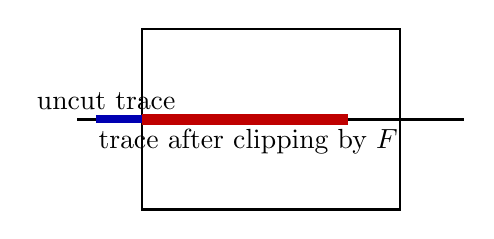
\begin{tikzpicture}[scale=.82]
  \draw[thick] (-2,-1.4) rectangle (2,1.4);
  \draw[very thick] (-3,0)--(3,0);
  \draw[blue!70!black,line width=3pt] (-2.7,0)--(1.2,0);
  \draw[red!75!black,line width=4pt] (-2,0)--(1.2,0);
  \node[above] at (-2.55,0) {uncut trace};
  \node[below] at (-.35,0) {trace after clipping by $F$};
\end{tikzpicture}

\caption{The same uncut open section can produce open, half-open, or closed
relative traces after intersection with the closed ambient section.}
\label{fig:clipping}
\end{figure}

\subsection{Lower-dimensional atoms}

Let $P_1$ be a rectangle, and let $P_2$ and $P_3$ be its upper and lower
halves with their common horizontal side retained only in the closed model.
Then the strict output code contains the word $\{1\}$ along that horizontal
segment, while the adjacent open regions carry $\{1,2\}$ and $\{1,3\}$.
This is an exact lower-dimensional atom.  No positive-radius witness is
available, but the open-to-closed argument retains the word through its line
trace.

\subsection{Simultaneous events}

If two neurons have a common trace endpoint $a$ on a prescribed line, the
representative package contains the same geometric point $a$ for both
closed sections.  The output therefore retains literal endpoint equality;
it does not merely preserve the two endpoint orders separately.  This is
what is needed when two face models must agree on a shared edge.
